\documentclass[11pt]{beamer}
\usetheme{Berkeley}
\usepackage[utf8]{inputenc}
\usepackage{amsmath}
\usepackage{amsfonts}
\usepackage{amssymb}
\usepackage{graphicx}

% für code
\usepackage{listings}
\usepackage{color}
\author{Sebastian Ruder}
\title{Construction and Analysis of an Emotion Proposition Store}
%\setbeamercovered{transparent} 
%\setbeamertemplate{navigation symbols}{} 
%\logo{} 
\institute{Institute of Computational Linguistics, University of Heidelberg} 
\date{21.07.15} 
%\subject{} 

\begin{document}

\begin{frame}
\titlepage
\end{frame}

\begin{frame}{Agenda}
\tableofcontents
\end{frame}

\section{Introduction}

\begin{frame}{Introduction}

\begin{itemize}
	\item Sentiment analysis (positive/negative/neutral) $\rightarrow $ important for many down-stream applications
	\item Emotion detection: subtask of sentiment analysis
	\item Project
	\begin{enumerate}
		\item Design and evaluation of frequent and clearly emotion-indicating patterns
		\item Acquisition of $>$ 1,700,000 propositions (emotion, emotion holder, cause) from Gigaword news corpus \cite{gigaword}
		\item Storage in an emotion proposition store
		\item Distributional analysis and evaluation for further insights (ambiguous concepts, etc.)
	\end{enumerate}
\end{itemize}

\end{frame}

\begin{frame}{Motivation}
	\begin{itemize}
		\item \textit{(I think) people are happy because Chavez has fallen.} \cite{benefactive_malefactive}; \textsc{E: fall(X)} is a bad-for event; \textsc{happy\_about(Y, E)} has a positive emotion $\rightarrow$ requires insights about emotion expressions over propositions, positively/negatively perceived events
		\item Resource for emotion detection
		\item Pattern-based approach can be extended to other domains
	\end{itemize}
\end{frame}

\section{Foundations}

\begin{frame}{Classification}
\begin{figure}[bth]
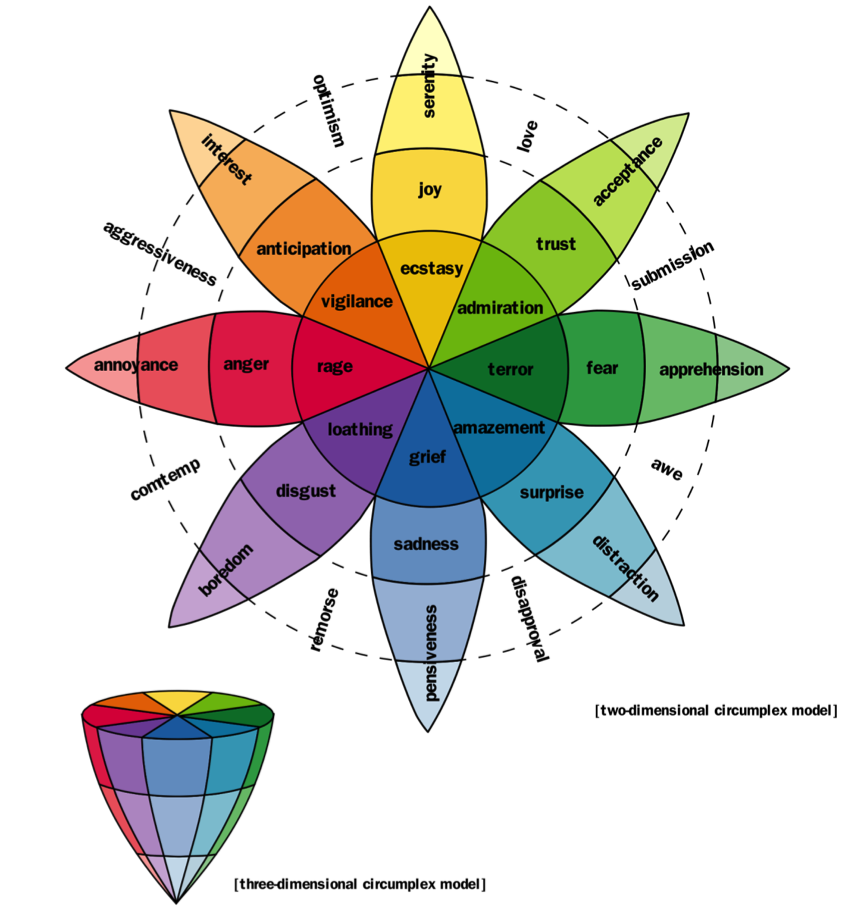
\includegraphics[width=.60\linewidth]{gfx/plutchik_wheel_emotion.png}
\caption{Plutchik's emotion wheel \cite{plutchik}}\label{fig:plutchik}
\end{figure}
\end{frame}

\begin{frame}{Emotions}
	\begin{itemize}
		\item Diverse linguistic triggers (\textit{disaster}, \textit{yucky}, \textit{betray})
		\item Compositionality (\textit{the blind} + \textit{sees})
		\item Semantic roles: Emotion holder \& cause
		\item Ambiguity
	\end{itemize}
$\rightarrow$ frequent \& clearly emotion indicating predicators, e.g. \textit{X be angry about NP / that S}, \textit{X fears that S} for acquisition	
\end{frame} 

\begin{frame}{Corpus}
\begin{itemize}
	\item Annotated Gigaword v.5 \cite{annotated_gigaword}
\end{itemize}

\begin{table}[h]
\centering
\begin{tabular}{l|l}
{\bf \# tokens} & {\bf \# documents}\\\hline
4,032,686,000   & 9,876,086
\end{tabular}
\caption{Number of tokens and documents for English Gigaword v.5}
\label{tab:gigaword}
\end{table}

\end{frame}

\section{Patterns}

\begin{frame}{Patterns}

\begin{align}
\begin{split}\label{ex:pattern_templates}
&\textnormal{fear	scare/Verb	NP	true}\\
&\textnormal{joy	be/Verb RB happy/JJ that/IN	S	false}
\end{split}
\end{align}

\begin{enumerate}
	\item \texttt{fear	(?! not)(?! never)scare/VB[DGPZ]/[0-9]+
	NP}
	\item \texttt{fear	(?<= )be/VB[PDGZ]/([0-9]+)(?! not)
	(?! never)( [a-z]+/RB/[0-9]+)?
	scare/VBN/[0-9]+ that/IN/[0-9]+	S}
	\item \texttt{fear	(?<= )be/VB[PDGZ]/([0-9]+)(?! not)
	(?! never)( [a-z]+/RB/[0-9]+)?
	scare/VBN/[0-9]+ by/IN/[0-9]+ NP}
	\item \texttt{joy	(?! not)(?! never)be/VB[DGPZ]/[0-9]+
	(?! not)(?! never)( [a-z]+/RB/[0-9]+)?
	happy/JJ/[0-9]+ that/IN/[0-9]+	S}
\end{enumerate}

\end{frame}

\begin{frame}{Pattern sources}
	
\begin{table}[]
\centering
\begin{tabular}{l|r}
{\bf Source}                 & {\bf \# of patterns} \\\hline
Oxford English Dictionary    & 24                   \\
Merriam-Webster's Dictionary & 51                   \\
Roget's Thesaurus            & 101                  \\
Harvard General Inquirer \cite{general_inquirer} & 0 \\
NRC Emolex \cite{nrc_emolex} & 0 \\
Emotion verb classes \cite{emotion_verbs}   & 24                   \\
Adjectives \cite{adjective_supersenses} & 126                  \\
VerbNet (\textit{admire} + \textit{amuse}) \cite{verbnet} & 178                  \\
FrameNet (\textsc{emotions} frame) \cite{framenet}                    & 173                  \\
WordNet-Affect \cite{wordnet-affect}     & 123                 
\end{tabular}
\caption{Overview of the productivity of sources for pattern design}
\label{tab:patterns-from-sources}
\end{table}
\end{frame}

\begin{frame}{Annotator agreement on most frequent patterns}

\begin{table}
\centering
\begin{tabular}{l|r}
Annotated expressions & Number\\\hline
Unanimous emotions & 106\\
Unanimous emotions (including 2nd choice) & 119\\
Majority emotions & 163\\
Unanimous emotions + degree & 39\\
Majority emotions + degree & 131\\\hline
\textit{Total} & 180\\\hline
Fleiss' $\kappa$ & 0.65
\end{tabular}
\caption{Number of annotated expressions for different forms of agreement}
\label{tab:annotation}
\end{table}
\end{frame}

\begin{frame}{Final pattern distribution across emotions}
\begin{table}[h]
\centering
\begin{tabular}{l|l}
{\bf Emotion} & {\bf \# of majority patterns} \\\hline
Joy           & 31\\
Trust         & 8\\
Fear          & 22\\
Surprise      & 16\\
Sadness       & 18\\
Disgust       & 14\\
Anger         & 29\\
Anticipation  & 25\\\hline
\textit{Total} & 163
\end{tabular}
\caption{Number of patterns that have been labeled by the majority with the same emotion}
\label{tab:pattern_emotion_distribution}
\end{table}
\end{frame}

\section{Extraction}

\begin{frame}{Extraction}
	\begin{itemize}
		\item Constituencies $<<$ dependencies
		\item Collapsed Stanford dependencies (\texttt{nsubj}, \texttt{dobj}, \texttt{conj\_and}, \texttt{ccomp}, \texttt{pcomp}, etc.)
		\item Modifiers (\texttt{nn}, \texttt{amod}, \texttt{num})
		\item Prepositional objects
		\item Coreference resolution
		\item Tagging of named entities
	\end{itemize}
\end{frame}

\begin{frame}{Extraction example}
	\begin{itemize}
	\item \textit{The countries had engaged in a multimillion-dollar battle to host the tournament, with Japan relying on its economic clout and South Korea relying on its superior soccer pedigree.}
	\item \texttt{NYT\_ENG\_19960601.0010/1	trust	rely on	Japan/LOCATION	economic clout					[its/PRP\$, economic/JJ, clout/NN]}
	\item \textit{The Japanese, who expected to win the right to host the tournament, were dismayed}.	
		\item \texttt{NYT\_ENG\_19960601.0010/9	anticipation	expect	Japanese				win	right		[to/TO, win/VB, the/DT, right/NN, to/TO, host/VB, the/DT, tournament/NN]}
	\end{itemize}
\end{frame}

\section{Analysis}

\begin{frame}{Emotion distribution}
		
\begin{table}[h]
\centering
\begin{tabular}{l|r|r|r}
{\bf Emotion} & {\bf Frequency} & {\bf\% of total} & {\bf\# of patterns with}\\ 
              &                 &   {\bf extractions}                           & {\bf 10+ occurrences}\\\hline
anticipation  & 966,571          & 54.47                       & 22 \\
fear          & 249,103          & 14.04                       & 20 \\
joy           & 231,967          & 13.07                       & 30 \\
trust         & 89,217           & 5.03                        &  6 \\
anger         & 64,586           & 3.64                        & 28 \\
surprise      & 60,221           & 3.39                        & 20 \\
disgust       & 59,486           & 3.35                        & 15 \\
sadness       & 53,269           & 3.00                        & 13\\\hline
Total         & 1,774,420         & 100.00                     & 154                
\end{tabular}
\caption{Frequencies of emotions in extractions}
\label{tab:extraction-emotion-freq}
\end{table}
\end{frame}

\begin{frame}{NP vs. S as cause}
\begin{table}[h]
\centering
\begin{tabular}{l|r|r}
{\bf Emotion} & {\bf \# extractions} & {\bf \# extractions} \\
{\bf }        & {\bf with NP cause}         & {\bf with S cause}          \\\hline
anticipation  & 407,738                & 558,833                \\
joy           & 190,484                & 41,483                 \\
fear          & 82,116                 & 166,987                \\
trust         & 72,483                 & 16,734                 \\
surprise      & 59,657                 & 564                    \\
disgust       & 58,942                 & 544                    \\
anger         & 57,379                 & 7,207                  \\
sadness       & 26,064                 & 27,205                 \\\hline
Total         & 956,392                &	819,557
\end{tabular}
\caption{Patterns with NP vs. S cause}
\label{tab:patterns-np-vs-s}
\end{table}

\end{frame}

\begin{frame}{PMI vs. chi-square}


\begin{table}[h]
\centering
\begin{tabular}{l|r|l|r}
{\bf $\chi^{2}$ bigram} & {\bf $\chi^{2}$ value} & {\bf PMI bigram}        & {\bf PMI} \\
& & & {\bf value}\\\hline 
loss of:life            & 9426.09                & death of:NUM         & 3.40            \\
loss of:innocent\_life  & 2317.45                & quake victim            & 3.37            \\
tragic loss             & 1430.38                & death of:wife           & 3.37            \\
loss of:civilian\_life  & 1416.05                & loss of:man             & 3.37            \\
civilian casualty       & 1303.09                & tragic loss             & 3.36            \\
death of:NUM            & 1208.49                & death of:father         & 3.36            \\
death of:NUM\_people & 1038.87                & death  & 3.34            \\
& & of:NUM\_people & \\
NUM victim           & 870.43                 & death of:relative       & 3.33            \\
unfortunate incident    & 677.81                 & loss of:friend          & 3.33            \\
choice of:word          & 516.71                 & innocent victim         & 3.33           
\end{tabular}
\caption{Comparison of $\chi^{2}$ and PMI values for the top 10 sadness NP cause bigrams}
\label{tab:chi-pmi sadness}
\end{table}
\end{frame}

\begin{frame}{Most ambiguous expressions}

\begin{figure}[bth]
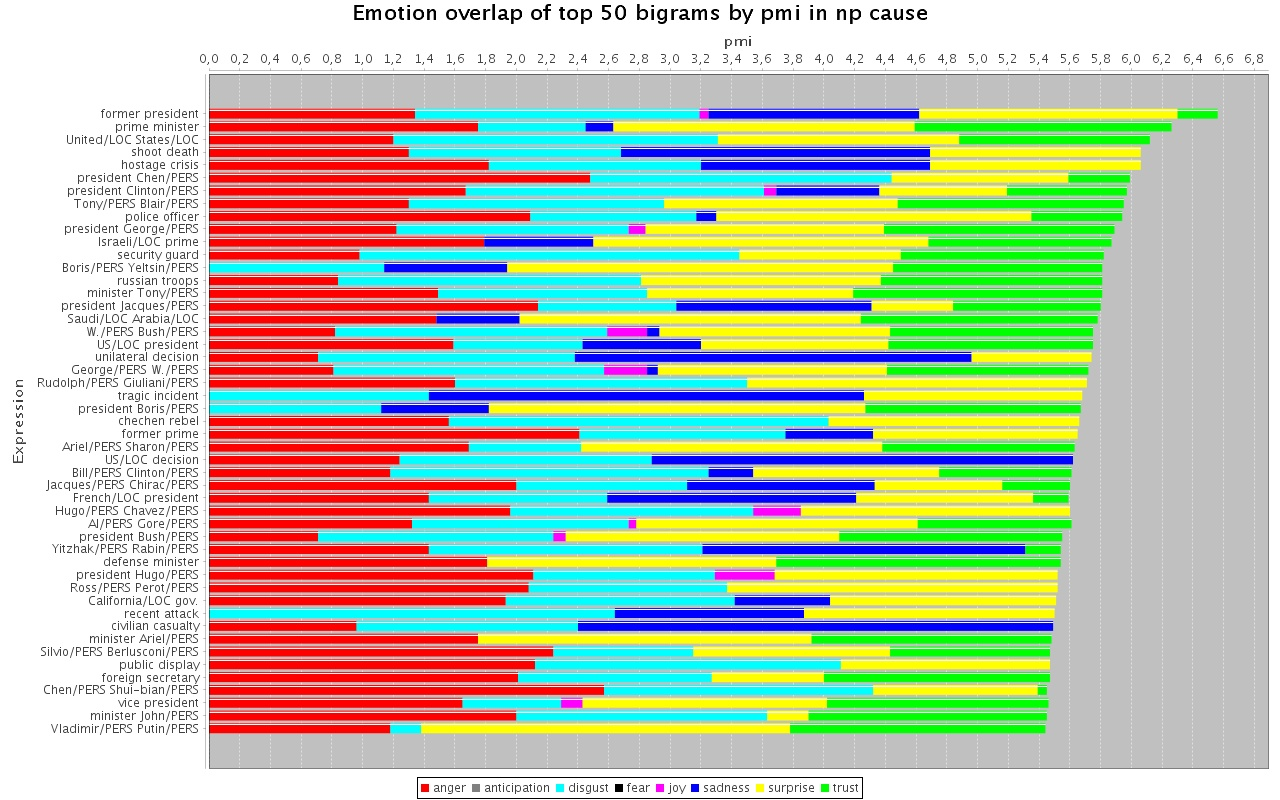
\includegraphics[width=\linewidth]{gfx/pmi_bigram_np_cause_emotion_overlap_50.jpg}
\caption{Overlap across emotions for the top 50 PMI NP cause bigrams}\label{fig:pmi-bigram-np-cause-emotion-overlap-50}
\end{figure}

\end{frame}

\begin{frame}{Agreement with NRC EmoLex}

\begin{figure}[bth]
\includegraphics[width=\linewidth]{gfx/pmi_np_cause_nrc_overlap_30.jpg}
\caption{Emotion and sentiment overlap of NP cause bigrams with the NRC Emotion Lexicon}\label{fig:pmi-np-cause-nrc-overlap}
\end{figure}

\end{frame}

\begin{frame}{Performance against annotated gold standard}
\begin{table}[]
\centering
\begin{tabular}{l|lll|lll}
\multicolumn{1}{c}{{\bf }} & \multicolumn{3}{c}{{\bf NP cause}} & \multicolumn{3}{c}{{\bf S cause pred + dobj}} \\
{\it Emotion/sentiment} & {\it P} & {\it R} & {\it F1} & {\it P} & {\it R} & {\it F1} \\\hline
anger & 0.00 & - & - & 0.00 & - & - \\
anticipation & 0.00 & - & - & 0.00 & - & - \\
disgust & 0.07 & 1.00 & 0.13 & 0.06 & 1.00 & 0.11\\
fear & 0.33 & 1.00 & 0.50 & 0.40 & 0.89 & 0.55\\
joy & 0.90 & 0.95 & 0.92 & 0.83 & 0.60 & 0.70\\
sadness & 1.00 & 0.67 & 0.80 & 0.36 & 0.45 & 0.40\\
surprise & 0.00 & - & - & 0.00 & - & - \\
trust & 0.00 & - & - & 0.05 & 1.00 & 0.10 \\\hline
\textit{total -- emotion} & 0.36 & 1.00 & 0.53 & 0.23 & 1.00 & 0.37\\\hline
positive & 0.56 & 0.96 & 0.71 & 0.40 & 0.57 & 0.47\\
negative & 0.60 & 0.84 & 0.70 & 0.37 & 0.87 & 0.51\\
neutral & 0.00 & - & - & 0.00 & - & - \\\hline
\textit{total -- sentiment} & 0.47 & 1.00 & 0.64 & 0.29 & 1.00 & 0.45
\end{tabular}
\caption{Precision, recall, and \textit{F1} score for emotions/sentiments of NP cause and S cause predicate + object bigrams}
\label{tab:bigrams-precision-against-annotation}
\end{table}
\end{frame}

\begin{frame}{Topic modeling}
\begin{itemize}
	\item LDA with different topic configurations (10, 20, 30, 50 topics) on 8 emotion-associated pseudo-documents
	\item Evaluation of how well topics are associated with certain emotions
\end{itemize}

\end{frame}

\section{Lessons learned}

\begin{frame}{Lessons learned}
	\begin{itemize}
		\item Amount of available data directly impacts results (only few S causes for surprise, disgust, anger)
		\item Different configuration produce a plethora of different scenarios that need to evaluated
		\item Finding adequate resources for evaluation can be difficult; manual annotation is expensive
	\end{itemize}
\end{frame}

\begin{frame}[allowframebreaks]{Bibliography}
\bibliographystyle{unsrt}
\bibliography{Bibliography}
\end{frame}

\end{document}%%%%%%%%%%%%%%%%%%%%%%%%%%%%%%%%%%%%%%%%%